\documentclass[a4paper,10pt]{article}


%%++++++++++++++++++++++++++++++++++++++++++++++++++++++++++++++++++++++++++++++
%%  Packages
\usepackage[english]{babel} 			% Langue
\usepackage[utf8]{inputenc}											% Encodage
\usepackage[T1]{fontenc}											  % Requis

\usepackage[pdftex]{graphicx}										% Images 
\usepackage{fancyhdr}												% Spécifier Entête et pieds.
\usepackage[margin=2.5cm]{geometry}

\usepackage{url}													% URL 
\usepackage{hyperref}
\usepackage{verbatim}												% Texte entre 	\begin{verbatim}  \end{verbatim} ne sera pas interprété
\usepackage{listliketab}											% List spéciale, notament comme tableau
\usepackage{longtable}
\usepackage{booktabs}												% Permet de faire des tableau plus avec des traits
% Exemple:
%\begin{tabular}{llr}
%\toprule
%\multicolumn{2}{c}{Item} \\
%\cmidrule(r){1-2}
%Animal & Description & Price (\$) \\
%\midrule
%Gnat  & per gram & 13.65 \\
%      & each     &  0.01 \\
%\bottomrule
%\end{tabular}

\usepackage{color}		
%% \definecolor{orange}{RGB}{255,127,0} http://en.wikibooks.org/wiki/LaTeX/Colors

\usepackage{tabularx}											% Tableau streatching 
\usepackage{colortbl}											% Permet des tableaux exotiquement colorier 
\usepackage{wrapfig}											% Permet d'alligner une figure à guache ou à droite
%\begin{wrapfigure}{r}{40mm}
%  \begin{center}
%    \includegraphics{toucan.eps}
%  \end{center}
%  \caption{The Toucan}
%\end{wrapfigure}
\usepackage{rotating}
\usepackage{amsmath}
\usepackage{subfig}
\usepackage{pdfpages}										% inclus pdf http://www-hep2.fzu.cz/tex/texmf-dist/doc/latex/pdfpages/pdf-ex.pdf
\usepackage[subfigure]{tocloft}
%\begin{figure}[htp]
%  \begin{center}
%    \subfigure[Original image]{\label{fig:edge-a}\includegraphics[scale=0.75]{toucan.eps}}
%    \subfigure[After Laplace edge detection]{\label{fig:edge-b}\includegraphics[scale=0.75]{laplace_toucan.eps}} \\
%    \subfigure[After Sobel edge detection]{\label{fig:edge-c}\includegraphics[scale=0.75]{sobel_toucan.eps}}
%  \end{center}
%  \caption{Various edge detection algorithms}
%  \label{fig:edge}
%\end{figure}
\usepackage[table]{xcolor}								
\usepackage{url}	
%\usepackage{lscape} 								%% Texte en landspcae
%\begin{landscape}
%notre texte
%\end{landscape}

%%++++++++++++++++++++++++++++++++++++++++++++++++++++++++++++++++++++++++++++++
%%  macros
\newcommand{\todo}[1]{\colorbox{red}{\color{white}:TODO:}#1}




\usepackage{color}
\usepackage{listings}



%%%%%%%%%%%%%%%%%%%%%%%%
%%  Design
%%%%%%%%%%%%%%%%%%%%%%%%%%
%%
%%  Pren1 Schlussdokument
%%  Kopf und Fusszeilen
%%  CT
%%
%%%%%%%%%%%%%%%%%%%%%%%%

\pagestyle{fancy}
  \renewcommand\headrulewidth{0.4pt}
  \fancyhf{}
  \setlength{\headheight}{35.60004pt}
%  \addtolength{\texthight}{-2*\headheight}
  \lhead{
    \protect
\includegraphics[height=32pt]{./images/model/eifr-logo.jpg}
  }
  \rhead{
    Mobile development TD3\\
   Jonathan Stoppani et Elias Medawar\\
  }
  \cfoot{
    \thepage
  }
\fancypagestyle{plain}{
  \renewcommand\headrulewidth{0.4pt}
  \fancyhf{}
  %\addtolength{\headheight}{\baselineskip}
  \lhead{
    \protect
\includegraphics[height=32pt]{./images/model/eifr-logo.jpg}
  }
  \rhead{
    Mobile development TD3\\
     Jonathan Stoppani et Elias Medawar\\
  }
  \cfoot{
  }
}
\fancypagestyle{empty}{
  \renewcommand\headrulewidth{0pt}
  \fancyhf{}
  %\addtolength{\headheight}{\baselineskip}
  \lhead{
  }
  \cfoot{
  }
}

\begin{document}
	\begin{titlepage}
	
	%\sffamily

		
	\addtolength{\leftskip}{-1cm}\addtolength{\rightskip}{-3.5cm}
	%\sffamily
	\vfill
	
	\hspace{0.10cm}	
\includegraphics{./images/model/eifr-logo.jpg} 

	\vfill
	\hspace{8.99cm}\Huge Mobile development  3 
	
	\hspace{9.08cm}\LARGE Report TD 3 : 
	      
	\vfill
	\Large
	
	\hspace{9.08cm}  Jonathan Stoppani et Elias Medawar
	
	\vfill
	\hspace{9.08cm}\normalsize Version:  \today
	\vfill
	\thispagestyle{empty}
	\clearpage

\end{titlepage}

	
	%%%%%%%%%%%%%%%%%%%%%%%%
%%
%%  Pren1 Schlussdokument
%%  Kopf und Fusszeilen
%%  CT
%%
%%%%%%%%%%%%%%%%%%%%%%%%

\pagestyle{fancy}
  \renewcommand\headrulewidth{0.4pt}
  \fancyhf{}
  \setlength{\headheight}{35.60004pt}
%  \addtolength{\texthight}{-2*\headheight}
  \lhead{
    \protect
\includegraphics[height=32pt]{./images/model/eifr-logo.jpg}
  }
  \rhead{
    Mobile development TD3\\
   Jonathan Stoppani et Elias Medawar\\
  }
  \cfoot{
    \thepage
  }
\fancypagestyle{plain}{
  \renewcommand\headrulewidth{0.4pt}
  \fancyhf{}
  %\addtolength{\headheight}{\baselineskip}
  \lhead{
    \protect
\includegraphics[height=32pt]{./images/model/eifr-logo.jpg}
  }
  \rhead{
    Mobile development TD3\\
     Jonathan Stoppani et Elias Medawar\\
  }
  \cfoot{
  }
}
\fancypagestyle{empty}{
  \renewcommand\headrulewidth{0pt}
  \fancyhf{}
  %\addtolength{\headheight}{\baselineskip}
  \lhead{
  }
  \cfoot{
  }
}
	
	\section{KVC  }
		\subsection{Source code in address for the KVC  ''request'' }
		\begin{center}
					 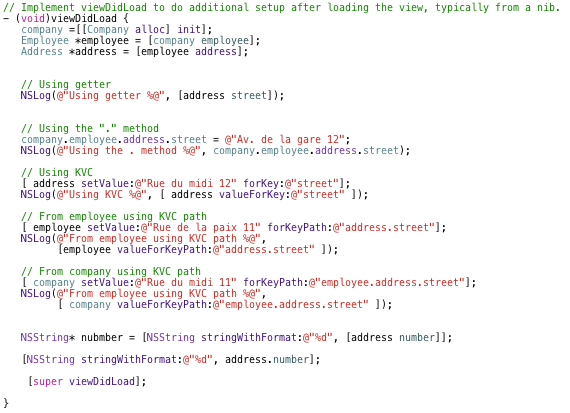
\includegraphics[width=1\textwidth]{./images/srcKVC.png}
		\end{center}
		\subsection{Output }
				\begin{center}
							 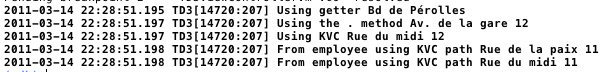
\includegraphics[width=1\textwidth]{./images/resultKVC.png}
				\end{center}
		\section{ KVO }
			\subsection{M file of the address with the int and numberDouble}	
				\begin{center}
				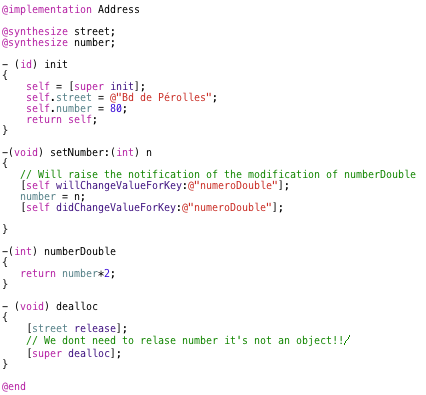
\includegraphics[scale=0.8]{./images/srcAddress.png}
				\end{center}
				The numberDouble is a calculated value so we have to raise ``manually `` the notifications.
			\subsection{H file of the address with the int and numberDouble}	
				\begin{center}
				 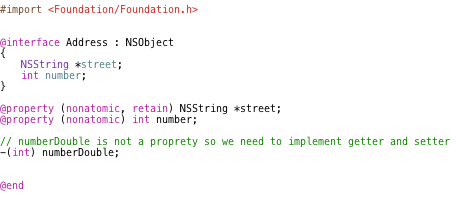
\includegraphics[scale=0.8]{./images/srcAddressH.png}
				\end{center}
			\subsection{UI with 2 text-field and a button}	
				\begin{center}
					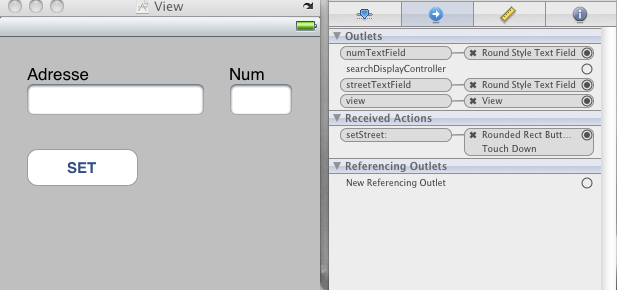
\includegraphics[width=1\textwidth]{./images/createGraphic.png}
				\end{center}
				Here we see the creation and links in \textbf{Interface builder}
			\subsection{Setting value of text fields}	
					\begin{center}
						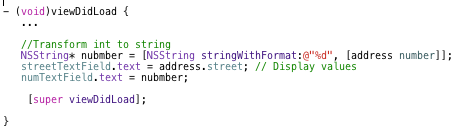
\includegraphics[scale=0.8]{./images/displayValue.png}
					\end{center}
				At the load of the application we set the value that will be displayed\\
				The conversion form int to string was found on this website: http://stackoverflow.com/questions/169925/how-to-do-string-conversions-in-objective-c
			\subsection{Result after loading}	
					\begin{center}
						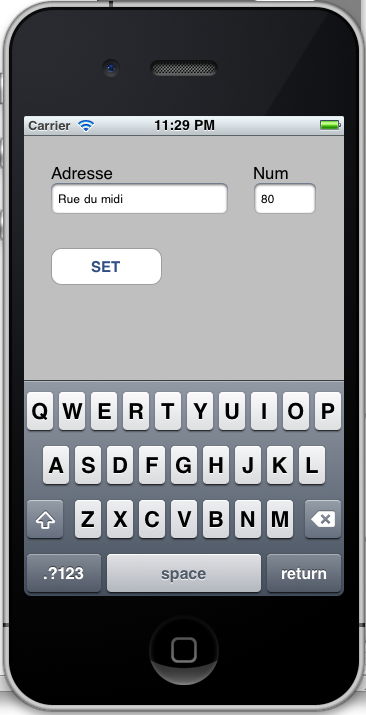
\includegraphics[scale=0.3]{./images/resutl1KVO.png}
					\end{center}
			\subsection{Registering and receiving the KVO notification in the employee class }
			\begin{center}
						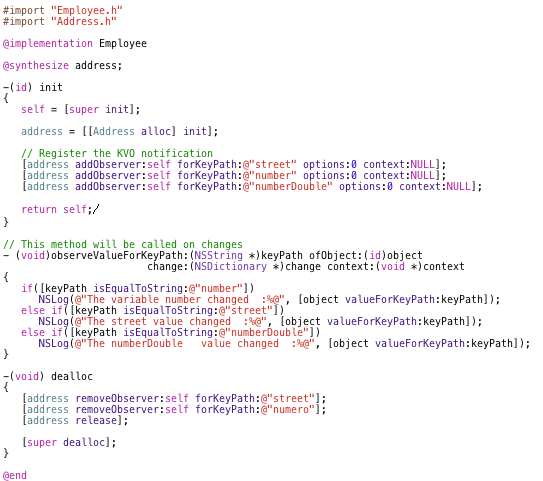
\includegraphics[scale=0.8]{./images/regrec.png}
			\end{center}
			We are responsible to unsubscribe the notification in the dealloc method. 
			\subsection{Result of the execution}
			\begin{center}
						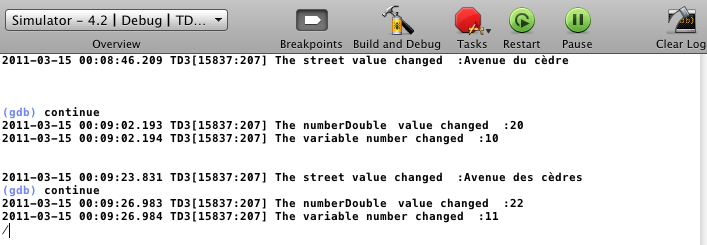
\includegraphics[scale=0.6]{./images/result2KVO.png}
			\end{center}
			1 .For this tests , we change at first the street value then press set\\
			2 The we change the number value and press set\\
			3 Finally we change both value and press set\\
			
			We tried to call just the didChangeValueForKey  in the setNumber method of the  address class.But the notification doesn't work without both call wil and didChangeValueForKey.
			
				\section{ Notifications }
						\subsection{M file of the company class}	
							\begin{center}
							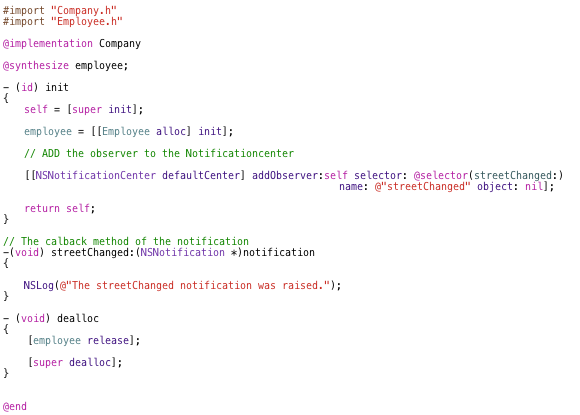
\includegraphics[scale=0.8]{./images/cmpSrc.png}
							\end{center}
						Here we have added an observer and the callback function to recive the specific information.
						
				\subsection{Raising notification }	
					\begin{center}
						 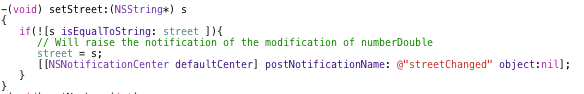
\includegraphics[scale=0.8]{./images/notCall.png}
					\end{center}
					In the address class when we change the value of the street we have to post a notification
					\subsection{Result }	
						\begin{center}
				 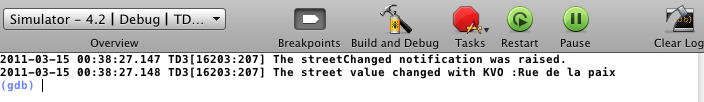
\includegraphics[scale=0.8]{./images/reslutNot.png}
						\end{center}
						The result in the console.
				
				\section{Conclusion}	
				KVC is very powerful but we have had some problem with the spelling of variable name. And this errors was not detected at the compilation time but at the run time.\\
				All the sources and documentation are available on gitHub at this address: \\ https://github.com/eia-fr/mobileDev/tree/master/TD3

\end{document}